
%=============================================================================
%
%	Project Euler 607
%
%=============================================================================



%=============================================================================
%	Packages
%=============================================================================

\documentclass[10pt, a4paper]{article}		% document format
\usepackage{graphicx}						% package to insert graphics
\usepackage[english]{babel}
\usepackage[utf8]{inputenc}					% this enables all unicode characters
\usepackage{amsmath, amsfonts, amssymb} 	% maths packages
\usepackage{amsthm}							% theorem styles
\usepackage{fancyhdr}						% package for headers, foot and matgin notes
\usepackage{enumitem}						% allows to change the enumeration format in line
\usepackage{mathtools}                      % useful math symbols like floor

\usepackage{tikz}                           % graphics package
\usepackage{pdflscape}



%=============================================================================
%	Commands
%=============================================================================

\providecommand{\U}[1]{\protect\rule{.1in}{.1in}}
\newcommand{\N}{\mathbb{N}}
\newcommand{\E}{\mathcal{E}}



%=============================================================================
%	Environment
%=============================================================================

\theoremstyle{plain}
\newtheorem{exercise}{Exercise}
\newtheorem{algorithm*}{Algorithm}

\theoremstyle{definition}
\newtheorem{solution}{Solution}[exercise]
\renewcommand*{\thesolution}{\theexercise.\alph{solution}}	% Make solution instances enumerate with number of exercise and letter of solution




%============================================================================
%	Pagestyle
%=============================================================================

\pagestyle{fancy}		% As we use the fancyhdr pkg need the fancy pagestyle, for more information:
						% http://tug.ctan.org/tex-archive/macros/latex/contrib/fancyhdr/fancyhdr.pdf


%\topmargin 0 pt
%\oddsidemargin 0 pt
%\evensidemargin 0 pt
%\marginparwidth 0 pt


%\textheight 25cm
%\textwidth 400 pt
%\advance\textheight by \topskip

%\parindent 0pt
%\parskip 5mm plus 1mm minus 1mm

%\fancyhead[C]{\textbf{el que sigui}}					% Central header
\fancyhead[L]{Project Euler 607}            			% Left header
\fancyhead[R]{Marc Jovani Bertran}						% Right header



%=============================================================================
%	Document
%=============================================================================

\begin{document}

\section*{Marsh Crossing}

\begin{center}
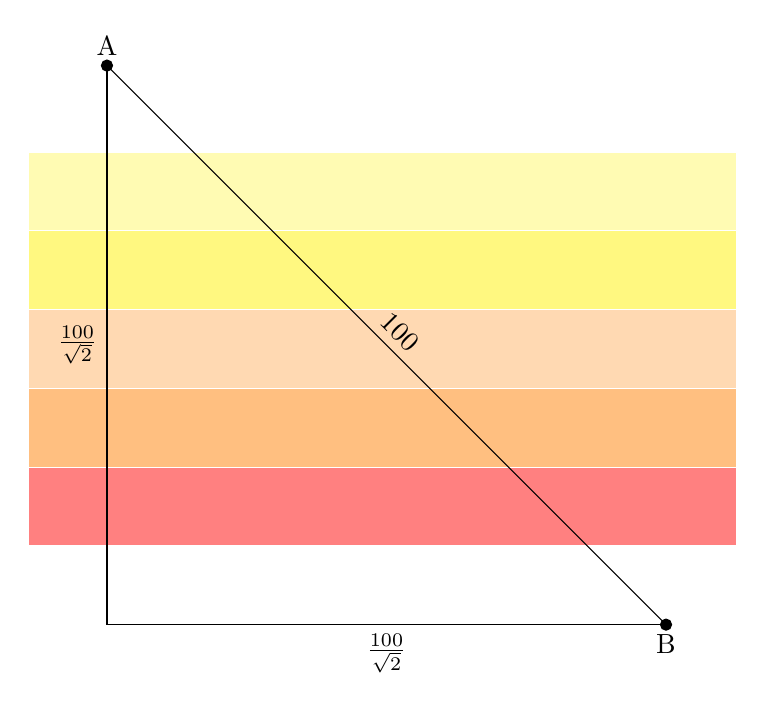
\begin{tikzpicture}
    \filldraw[fill=yellow!30!white, draw=white] (-1,6) rectangle (8,5);
    \filldraw[fill=yellow!50!white, draw=white] (-1,5) rectangle (8,4);
    \filldraw[fill=orange!30!white, draw=white] (-1,4) rectangle (8,3);
    \filldraw[fill=orange!50!white, draw=white] (-1,3) rectangle (8,2);
    \filldraw[fill=red!50!white, draw=white] (-1,2) rectangle (8,1);

    \draw[-] (0,0) -- (7.1,0) coordinate (x axis)
        node[pos=0.5, below] {$\frac{100}{\sqrt{2}}$};
    \draw[-] (0,7.1) -- (0,0) coordinate (x axis)
        node[pos=0.5, left] {$\frac{100}{\sqrt{2}}$};
    \draw[-] (0,7.1) -- (7.1,0) coordinate (x axis)
        node[pos=0.5, above, sloped] {100};

    \filldraw (0,7.1) circle (2pt) node(a)[align=left,   above] {A};
    \filldraw (7.1,0) circle (2pt) node(b)[align=left,   below] {B};
\end{tikzpicture}
\end{center}

The idea is to choose the values on the $x$ axis for each start/end of marsh zone and minimize the time travelled, while maintaining the values for the $y$ axis cosntant.

To do so the function we get is:

\begin{equation}
    \begin{aligned}
        f (x_1, x_2, x_3, x_4, x_5, x_6)
        & = \frac{\sqrt{(y_0 - y_1)^2 + (x_1 - x_0)^2}}{10}\\
        & + \frac{\sqrt{(y_1 - y_2)^2 + (x_2 - x_1)^2}}{9}\\
        & + \frac{\sqrt{(y_2 - y_3)^2 + (x_3 - x_2)^2}}{8}\\
        & + \frac{\sqrt{(y_3 - y_4)^2 + (x_4 - x_3)^2}}{7}\\
        & + \frac{\sqrt{(y_4 - y_5)^2 + (x_5 - x_4)^2}}{6}\\
        & + \frac{\sqrt{(y_5 - y_6)^2 + (x_6 - x_5)^2}}{5}\\
        & + \frac{\sqrt{(y_6 - y_7)^2 + (x_7 - x_6)^2}}{10}\\
    \end{aligned}
\end{equation}

As we see its a quadratic equation so we will use the Newtons method to solve the problem.

The gradient is:

\begin{equation*}
    \nabla f (x_1, x_2, x_3, x_4, x_5, x_6) = \left[
    \begin{aligned}
        &   \frac{x_1 - x_0}{10\sqrt{(y_0 - y_1)^2 + (x_1 - x_0)^2}}
            - \frac{x_2 - x_1}{9\sqrt{(y_1 - y_2)^2 + (x_2 - x_1)^2}}\\
        &   \frac{x_2 - x_1}{9\sqrt{(y_1 - y_2)^2 + (x_2 - x_1)^2}}
            - \frac{x_3 - x_2}{8\sqrt{(y_2 - y_3)^2 + (x_3 - x_2)^2}}\\
        &   \frac{x_3 - x_2}{8\sqrt{(y_2 - y_3)^2 + (x_3 - x_2)^2}}
            - \frac{x_4 - x_3}{7\sqrt{(y_3 - y_4)^2 + (x_4 - x_3)^2}}\\
        &   \frac{x_4 - x_3}{7\sqrt{(y_3 - y_4)^2 + (x_4 - x_3)^2}}
            - \frac{x_5 - x_4}{6\sqrt{(y_4 - y_5)^2 + (x_5 - x_4)^2}}\\
        &   \frac{x_5 - x_4}{6\sqrt{(y_4 - y_5)^2 + (x_5 - x_4)^2}}
            - \frac{x_6 - x_5}{5\sqrt{(y_5 - y_6)^2 + (x_6 - x_5)^2}}\\
        &   \frac{x_6 - x_5}{5\sqrt{(y_5 - y_6)^2 + (x_6 - x_5)^2}}
            - \frac{x_7 - x_6}{10\sqrt{(y_6 - y_7)^2 + (x_7 - x_6)^2}}\\
    \end{aligned}
    \right]
\end{equation*}

And the hessian:

\begin{equation*}
    \mathbf{H}_f
    \begin{bmatrix}
        & A_0 + A_1
        & A_1
        & 0
        & 0
        & 0
        & 0
        \\

        & A_1
        & A_1 + A_2
        & A_2
        & 0
        & 0
        & 0
        \\

        & 0
        & A_2
        & A_2 + A_3
        & A_3
        & 0
        & 0
        \\

        & 0
        & 0
        & A_3
        & A_3 + A_4
        & A_4
        & 0
        \\

        & 0
        & 0
        & 0
        & A_4
        & A_4 + A_5
        & A_5
        \\

        & 0
        & 0
        & 0
        & 0
        & A_5
        & A_5 + A_6
        \\

    \end{bmatrix}
\end{equation*}

where

\begin{equation*}
    A_i = \frac{cy_i}{s_i (cy_i + (x_{i + 1} - x_i)^2)^{\frac{3}{2}}}
\end{equation*}

Applying the Newtons method to find the zero of the gradient and so find the minumum we end up with this path:

\begin{center}
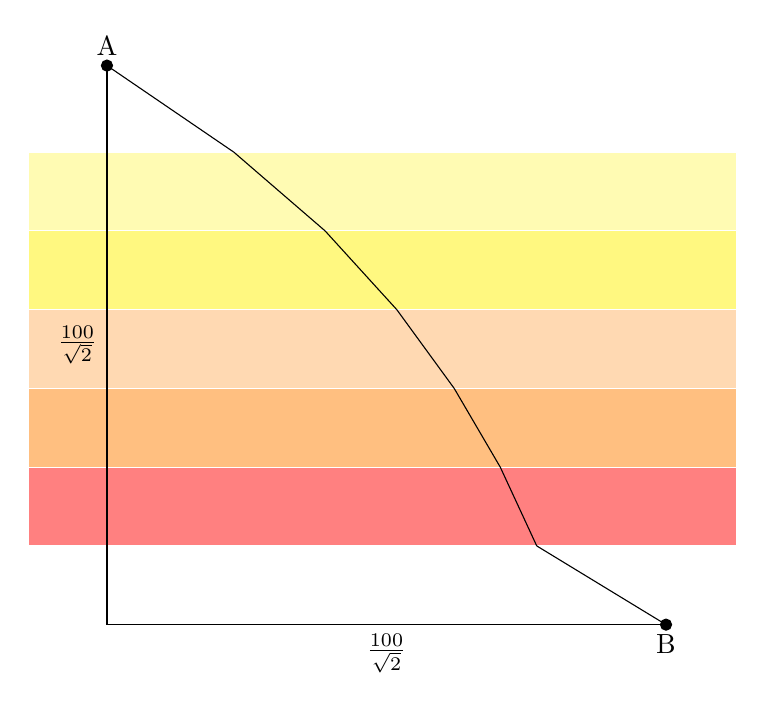
\begin{tikzpicture}
    \filldraw[fill=yellow!30!white, draw=white] (-1,6) rectangle (8,5);
    \filldraw[fill=yellow!50!white, draw=white] (-1,5) rectangle (8,4);
    \filldraw[fill=orange!30!white, draw=white] (-1,4) rectangle (8,3);
    \filldraw[fill=orange!50!white, draw=white] (-1,3) rectangle (8,2);
    \filldraw[fill=red!50!white, draw=white] (-1,2) rectangle (8,1);

    \draw[-] (0,0) -- (7.1,0) coordinate (x axis)
        node[pos=0.5, below] {$\frac{100}{\sqrt{2}}$};
    \draw[-] (0,7.1) -- (0,0) coordinate (x axis)
        node[pos=0.5, left] {$\frac{100}{\sqrt{2}}$};

    \filldraw (0,7.1) circle (2pt) node(a)[align=left,   above] {A};
    \filldraw (7.1,0) circle (2pt) node(b)[align=left,   below] {B};

    \draw[-] (0,7.1) -- (1.612,6) coordinate (x axis);
    \draw[-] (1.612,6) -- (2.771,5) coordinate (x axis);
    \draw[-] (2.771,5) -- (3.681,4) coordinate (x axis);
    \draw[-] (3.681,4) -- (4.41,3) coordinate (x axis);
    \draw[-] (4.41,3) -- (4.995,2) coordinate (x axis);
    \draw[-] (4.995,2) -- (5.458,1) coordinate (x axis);
    \draw[-] (5.458,1) -- (7.1,0) coordinate (x axis);
\end{tikzpicture}
\end{center}

Newtons method:

\begin{equation*}
    x_{k+1} = x_k - \frac{\nabla f(x_k)}{\mathbf{H}_f(x_k)}
\end{equation*}

To find the next point we need the inverse of the hessian, but as it might be too expencive we solve the linear sistem

\begin{equation*}
    \mathbf{H}_f(x_k) x = - \nabla f(x_k)
\end{equation*}

Where $x = x_{k+1} - x_k$. So we solve the sistem with gauss method and then compute the next $x$ with a small step to not go too far away and diverge from the solution.

\end{document}
